\chapter{系统设计}

基于需求分析,该部分介绍异构计算平台的系统设计。该部分按照自上而下的顺序,如图\ref{platform_arch}所示,分别介绍接口的设计,平台设计,工具链设计,和平台的系统环境设计。

\begin{figure}[h!]
    \centering
    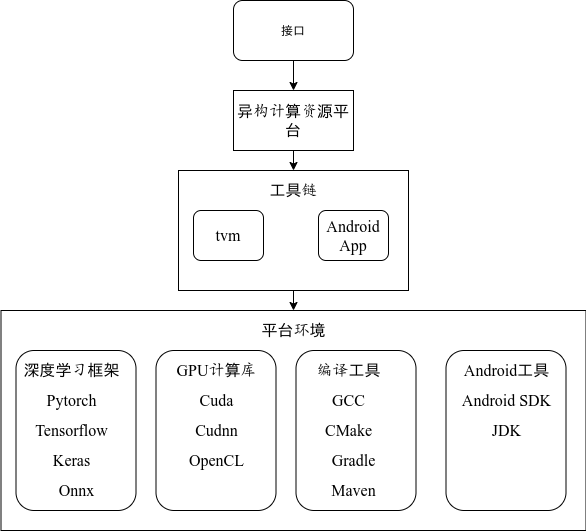
\includegraphics[width=180bp]{figure/platform_arch.png}
    \caption{系统架构}
    \label{platform_arch}
\end{figure}


\section{接口设计}

接口是平台暴露给用户使用API,与用户进行直接的交互,用户通过调用该API来进行模型的部署。

\begin{figure}[h!]
    \centering
    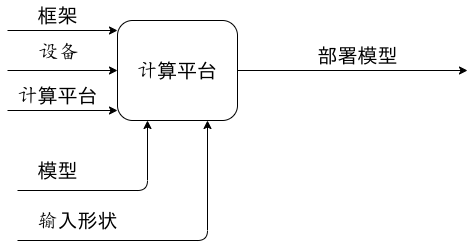
\includegraphics[width=180bp]{figure/platform_interface.png}
    \caption{系统接口}
    \label{platform_interface}
\end{figure}

平台通过把每种设备的部署抽象为一个类来实现相应的功能,通过一些参数来与用户交互。如上图\ref{platform_interface}所示,其中:
\begin{itemize}
    \item {框架参数:用户待部署的模型使用的深度学习框架。支持Pytorch,Tensorflow,Keras,Onnx。}
    \item {设备参数:用户部署的目标设备。支持本地,安卓设备,树莓派,VTA等。}
    \item {计算平台参数:用户部署需要使用的计算平台,此参数与具体的部署设备相关。本地支持CPU和Cuda,安卓设备支持CPU,OpenCL和Vulkan等。树莓派和VTA支持CPU。}
    \item {模型参数:是用户待部署的模型对象。}
    \item {输入形状参数:是用户模型输入向量的形状。}
\end{itemize}

通过该接口,用户最终得到部署后的模型对象,该对象可以像其他模型一样,计算输出。



\section{平台设计}

异构计算资源平台由几个部分组成:
\begin{itemize}
    \item {编译模块:把用户输入的模型编译为计算图的中间表示,把多种框架的不同计算图编译为统一的中间形式方便后续的部署。}
    \item {部署模块:把得到的计算图中间表示生成能够在具体硬件执行的动态链接库,能够部署到对应的平台执行推理。}
    \item {接口的实现:把接口实现为Python的类,在接口中封装编译和部署的功能,通过暴露出参数,来让用户调用。}
\end{itemize}


\section{工具链设计}

平台通过基于第三方的工具来辅助实现平台的功能。本项目中将会使用TVM和Android Rpc App(安卓RPC通信应用)以及VTA Simulator(VTA模拟器)来完成平台的功能。

TVM是一个端到端的神经网络模型的编译器工具链,支持目前主流的前端的深度学习框架,如Pytorch,Tensorflow,Onnx等,同时支持部署到广泛的后端硬件设备,如CPU,服务器端GPU,移动端GPU,FPGA等。所以,本项目采用TVM来实现模型的编译和部署。

其次,为了能够部署到安卓设备,需要主机和安卓设备进行通信,所以使用Android Rpc App来使主机和安卓设备进行通信,能够把模型上传到安卓设备。

最后,为了能够把模型部署到VTA上,在TVM生成VTA指令集的代码后,需要通过VTA模拟器来执行生成的可执行代码。


\section{平台环境设计}

平台系统环境指的是该平台依赖的所有底层软件和操作系统的总和。实现该平台需要依赖复杂的软件。其中包括深度学习框架,Pytorch,Tensorflow,keras,Onnx等。GPU计算库,Cuda,Cudnn,OpenCL等。编译工具GCC,CMake,Gradle,Maven等。构建Android App需要的JDK和Android SDK等。